\chapter{SPI sučelje i DMA prijenos}

SPI (engl. \textit{Serial Peripheral Interface}) protokol se koristi za prijenos podataka između \textit{flash} memorije i mikrokontrolera, odnosno međuspremnika kamere. Kako bi se oslobodili resursi na mikrokontroleru, za prijenos podataka između kamere i \textit{flash} memorije se, u kombinaciji sa SPI protokolom, koristi i DMA (engl. \textit{Direct Memory Access}) prijenos. S obzirom na to da se koriste \textit{Low-Layer} biblioteke, potrebno je razumjeti način rada SPI i DMA periferija mikrokontrolera. U ovom poglavlju bit će opisan SPI protokol i DMA prijenos i bit će istaknute razlike i problemi kod prilagođavanja programske podrške za STM32L471VGT6 mikrokontroler.

\section{SPI protokol}

SPI je sinkrono serijsko komunikacijsko sučelje koje se koristi za komunikaciju na kratkim udaljenostima, pretežito u ugradbenim računalnim sustavima \cite{spi_wikipedia}. 

SPI uređaji komuniciraju u \textit{full-duplex} načinu rada koristeći \textit{master-slave} arhitekturu, obično sa jednim \textit{master} uređajem. \textit{Master} (upravljač) uređaj proizvodi okvir za čitanje i pisanje. Više \textit{slave} uređaja može biti spojeno na jedan upravljač tako da se aktivira određeni \textit{chip select} signal za pojedini uređaj.

\subsection{Opis sučelja}

SPI sabirnica se sastoji od četiri signala:
\begin{itemize}
	\item SCLK: Serijski takt (izvor je \textit{master} uređaj)
	\item MOSI: \textit{Master Output Slave Input} (izvor podataka iz \textit{master} uređaja)
	\item MISO: \textit{Master Input Slave Output} (izvor podataka iz \textit{slave} uređaja)
	\item CS/SS: \textit{Chip/Slave Select} (aktivan nisko, signal iz \textit{master} uređaja, označava da se prenose podaci)
\end{itemize}
MOSI na \textit{master} uređaju se spaja na MOSI na \textit{slave} uređaju, dok se MISO na \textit{master} uređaju se spaja na MISO na \textit{slave} uređaju. CS/SS se koristi za pokretanje komunikacije između \textit{slave} i \textit{master} uređaja. Za svaki \textit{slave} uređaj postoji zaseban CS/SS priključak na \textit{master} uređaju. Takav način spajanja se naziva neovisni \textit{slave} uređaj. Primjer spajanja tri \textit{slave} uređaja na jedan \textit{master} uređaj u konfiguraciji neovisnog \textit{slave} uređaja prikazan je na slici \ref{fig:spi_three_slaves}.
\begin{figure}[H]
	\centering
	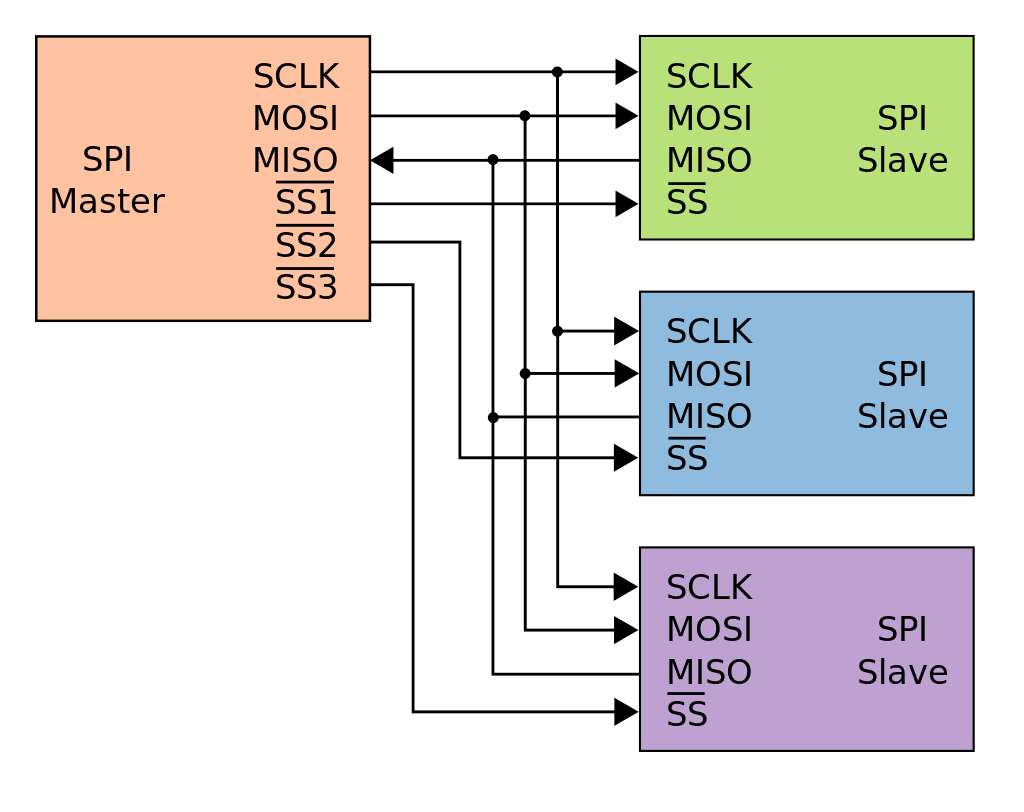
\includegraphics[height=7 cm]{SPI_three_slaves.svg.png}
	\caption{Spoj tri \textit{slave} uređaja na jedan \textit{master} uređaj u konfiguraciji neovisnog \textit{slave} uređaja. Vidljivo je da \textit{master} uređaj ima tri SS priključka, a svaki odgovara jednom \textit{slave} uređaju, dok se SCLK, MOSI i MISO linije međusobno dijele između \textit{slave} uređaja \cite{spi_wikipedia}}
	\label{fig:spi_three_slaves}
\end{figure}
Moguće je još spojiti uređaje u konfiguraciju ulančavanog \textit{slave} uređaja. U toj konfiguraciji \textit{slave} uređaji dijele isti CS/SS, a ulančavanjem preko MISO/MOSI linija podaci se prenose prema načelu posmačnog registra, koji je objašnjen u sljedećem potpoglavlju. Prikaz spajanja tri \textit{slave} uređaja se nalazi na slici \ref{fig:SPI_three_slaves_daisy_chained}.
\begin{figure}[H]
	\centering
	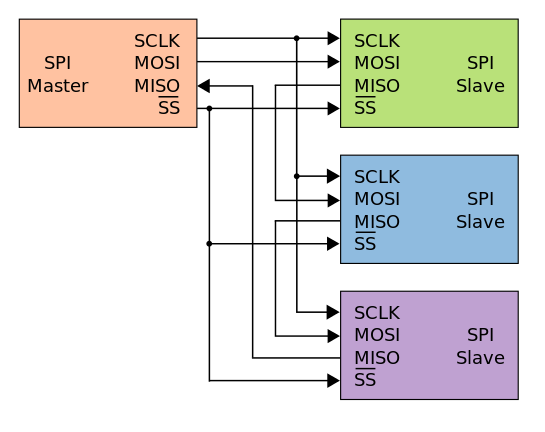
\includegraphics[height=7 cm]{SPI_three_slaves_daisy_chained.svg.png}
	\caption{Spoj tri \textit{slave} uređaja na jedan \textit{master} uređaj u konfiguraciji ulančavanog \textit{slave} uređaja \cite{spi_wikipedia}}
	\label{fig:SPI_three_slaves_daisy_chained}
\end{figure}

\subsection{Način rada}

SPI sabirnica radi s jednim \textit{master} uređajem i jednim ili više \textit{slave} uređaja. Ako se koristi jedan \textit{slave} uređaj, onda CS signal može biti postavljen u nisku logičku razinu, ako \textit{slave} uređaj to dopušta. Neki \textit{slave} uređaji zahtijevaju padajući brid CS signala kako bi započela komunikacija. Ako se koristi više \textit{slave} uređaja potreban je zaseban CS signal \textit{master} uređaja za svaki \textit{slave} uređaj.

\subsubsection{Prijenos podataka}

Za početak komunikacije \textit{master} uređaj konfigurira takt koristeći frekvenciju koju podržava \textit{slave} uređaj, obično do nekoliko MHz. \textit{Master} uređaj zatim odabire \textit{slave} uređaj postavljanjem CS linije u nisko logičko stanje. Ako je potreban period čekanja, npr. za AD (analogno-digitalnu) pretvorbu, \textit{master} uređaj mora pričekati minimalno taj period vremena prije puštanja takta.

Tijekom svakog perioda takta obavlja se prijenos podataka u \textit{full-duplex} načinu rada. To znači da \textit{master} uređaj pošalje jedan bit na MOSI liniju, koji \textit{slave} uređaj pročita, dok u isto vrijeme \textit{slave} uređaj šalje jedan bit na MISO liniju, koji \textit{master} uređaj pročita. Takva sekvenca se održava čak i kada se izvodi jednosmjerni prijenos podataka.

Prijenosi podataka uključuju dva posmačna registra zadane veličine, npr. 8 bitova, jedan u \textit{master} i drugi u \textit{slave} uređaju. Registri su spojeni u topologiji virtualnog prstena (slika \ref{fig:spi_circular_transfer}).
\begin{figure}[H]
	\centering
	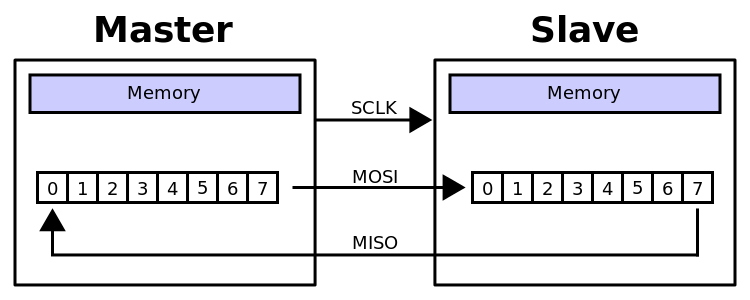
\includegraphics[width=\textwidth]{SPI_8-bit_circular_transfer.svg.png}
	\caption{Tipičan spoj dvaju posmačna registra koji formiraju kružni međuspremnik \cite{spi_wikipedia}}
	\label{fig:spi_circular_transfer}
\end{figure}
Podaci se obično pomiču tako da se prvo pomakne najznačajniji bit. Na brid takta, \textit{master} i \textit{slave} uređaj pomaknu bit i pošalju ga na prijenosnu liniju. Na sljedeći brid takta, na svakom prijamniku bit se uzorkuje s prijenosne linije i postavlja se kao novi najmanje značajni bit u posmačnom registru. \textit{Master} i \textit{slave} uređaji u potpunosti razmjene podatke u registrima nakon što se svi bitovi u registrima prebace. Ako je potrebno razmijeniti još podataka, posmačni registri se ponovno napune te se postupak ponavlja, a prijenos se može obavljati za bilo koji broj perioda takta. Kada je prijenos dovršen, \textit{master} uređaj prestaje davati takt i obično isključi CS signal, odnosno postavi ga na visoku razinu.

Prijenos se obično obavlja u riječima širine 8 bitova, no moguća je i širina riječi od 12 bita, ili čak 12 bitova, koji se koristi za digitalno-analogne i analogno-digitalne pretvornike.

\subsubsection{Polaritet takta i faza}

Osim što mora podesiti frekvenciju takta, \textit{master} uređaj mora isto tako podesiti polaritet takta (CPOL, engl. \textit{Clock Polarity}) i fazu (CPHA, engl. \textit{Clock Phase}) ovisno o podacima. Vremenski dijagram je prikazan na slici \ref{fig:spi_timing_diagram}.
\begin{figure}[H]
	\centering
	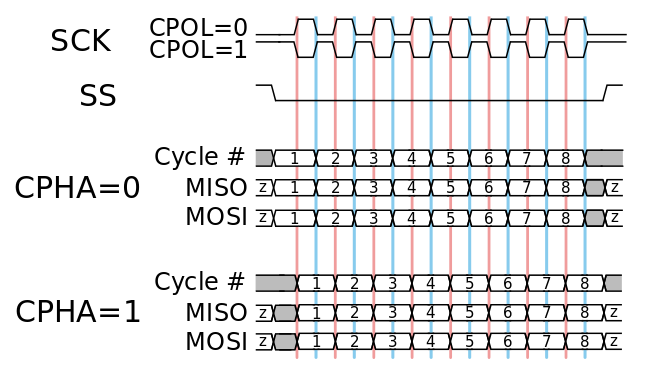
\includegraphics[height=7 cm]{SPI_timing_diagram2.svg.png}
	\caption{Vremenski dijagram koji pokazuje polaritet takta i fazu. Crvene linije označuju vodeće bridove, a plave linije označavaju prateće bridove.}
	\label{fig:spi_timing_diagram}
\end{figure}
CPOL određuje polaritet kanala. Polaritet može biti invertiran jednostavnim inverterom.
\begin{itemize}
	\item Ako je CPOL = 0, onda takt miruje u niskom logičkom stanju, a svaki period se sastoji od impulsa visokog logičkog stanja. To znači da je vodeći brid rastući brid, a prateći brid padajući brid.
	\item Ako je CPOL = 1, onda takt miruje u visokom logičkom stanju, a svaki period se sastoji od impulsa niskog logičkog stanja. To znači da je vodeći brid padajući brid, a prateći brid rastući brid.
\end{itemize}
CPHA određuje fazu podatkovnih bitova u odnosu na takt.
\begin{itemize}
	\item Ako je CPHA = 0, "izlazna" strana mijenja podatak na prateći brid prethodnog perioda takta, dok "ulazna" strana prihvaća podatak na (ili ubrzo nakon) vodeći brid perioda takta. Izlazna strana zadržava valjani podatak sve do pojave pratećeg brida trenutnog perioda takta.
	\item Ako je CPHA = 1, "izlazna" strana mijenja podatak na vodeći brid trenutnog perioda takta, dok "ulazna" strana prihvaća podatak na (ili ubrzo nakon) pratećeg brida perioda takta. Izlazna strana zadržava valjani podatak do pojave vodećeg brida sljedećeg perioda takta. Na zadnji period, \textit{slave} uređaj zadržava valjani podatak na MISO liniji sve dok \textit{slave} uređaj ne bude deselektiran.
\end{itemize}
MOSI i MISO signali su obično stabilni za vrijeme pola perioda takta, sve do sljedeće promjene takta. SPI \textit{master} i \textit{slave} uređaji mogu uzorkovati podatke u bilo kojem vremenu unutar te polovice periode takta.

Kombinacije različitih konfiguracija CPOL i CPHA bitova predstavljaju načine rada. Konvnecija je da CPOL predstavlja viši bit, dok CPHA predstavlja niži bit. Načini rada kod ARM-ovih mikrokontrolera su prikazani u tablici \ref{Tab:spi_modes}
\begin{center}
	\begin{table}[H]
		\centering
		\begin{tabular}{| c | c | c |}
			\hline
			SPI način rada & CPOL & CPHA \\
			\hline
			0 & 0 & 0 \\
			\hline
			1 & 0 & 1 \\
			\hline
			2 & 1 & 0 \\
			\hline
			3 & 1 & 1 \\
			\hline
		\end{tabular}
		\caption{SPI načini rada kod ARM-ovih mikrokontrolera \cite{spi_wikipedia}}
		\label{Tab:spi_modes}
	\end{table}
\end{center}

\section{DMA prijenos}